\documentclass[11pt,a4paper]{article}
\usepackage[T1]{fontenc}
\usepackage[utf8]{inputenc}
\usepackage[french]{babel}
\usepackage{lmodern,geometry,graphicx,booktabs,array,hyperref}
\geometry{margin=2.25cm}
\hypersetup{colorlinks=true,urlcolor=black,linkcolor=black}
\setlength{\parindent}{0pt}
\setlength{\parskip}{0.45em}
\renewcommand{\arraystretch}{1.16}

\begin{document}
\begin{center}
{\Large\bfseries Pipeline Big Data : données YouTube\par}
\vspace{0.25em}
{\large Rapport d'avancement -- semaine 1\par}
\vspace{0.55em}
Taha Hajji \quad Bouaicha Ibrahim \quad Ayoub Chenguir\\
Module Big Data Plateformes et Big Data Analytics
\end{center}

\section{Sujet retenu}

Le projet porte sur des vidéos YouTube correspondant à une requête choisie. Notre première requête de travail est \og big data maroc \fg{}. Nous cherchons à collecter des métadonnées et des statistiques publiques, puis à suivre leurs relevés dans le temps. Cette idée permet de construire une voie froide pour l'analyse historique et, plus tard, de définir une tâche de prédiction. Le sujet et les données doivent encore être validés par l'enseignante avant de fixer définitivement la cible du modèle.

Une observation est un \emph{instantané} d'une vidéo. Son identifiant est \texttt{video\_id} ; \texttt{collected\_at} indique quand les chiffres ont été relevés. Cela évite de confondre la date de publication d'une vidéo avec la date de mesure de ses vues. Une nouvelle collecte de la même vidéo produit un nouvel instantané, car les statistiques peuvent changer.

\begin{center}
\small
\begin{tabular}{p{4.5cm}p{9.4cm}}
\toprule
Champ & Rôle dans le projet \\
\midrule
\texttt{video\_id}, \texttt{collected\_at} & Identification de la vidéo et du relevé. \\
\texttt{published\_at} & Date de mise en ligne, utile pour les regroupements temporels. \\
\texttt{channel\_id}, \texttt{channel\_title} & Regroupement par chaîne. \\
\texttt{view\_count}, \texttt{like\_count}, \texttt{comment\_count} & Statistiques publiques ; une valeur peut être absente. \\
\texttt{title}, \texttt{category\_id}, \texttt{duration\_iso8601} & Description de la vidéo. \\
\texttt{query} & Requête de recherche ayant amené la vidéo dans le lot. \\
\bottomrule
\end{tabular}
\end{center}

L'API YouTube Data v3 est interrogée en deux temps : \texttt{search.list} fournit des identifiants, puis \texttt{videos.list} complète les champs retenus. Le script suit \texttt{nextPageToken}, supprime les identifiants répétés et interroge les détails par lots de 50. Le nombre de pages et le plafond de vidéos sont configurables ; la configuration actuelle limite le lot à 1\,000 vidéos. La clé API est lue depuis l'environnement local et ne figure pas dans le dépôt.

\section{Infrastructure préparée}

Le cluster est décrit dans \texttt{docker-compose.yml}. Il comprend un broker Kafka, un master Spark, deux workers Spark, un NameNode et deux DataNodes. Chaque DataNode dispose de son propre volume ; la configuration HDFS prévoit deux copies de chaque bloc. Pour les essais, chaque worker Spark est limité à un cœur et 512~Mo. Les images déjà présentes sur le poste ont été utilisées : Kafka 3.8.1, Spark 3.5.3 et Hadoop 3.2.1.

\begin{figure}[htbp]
\centering
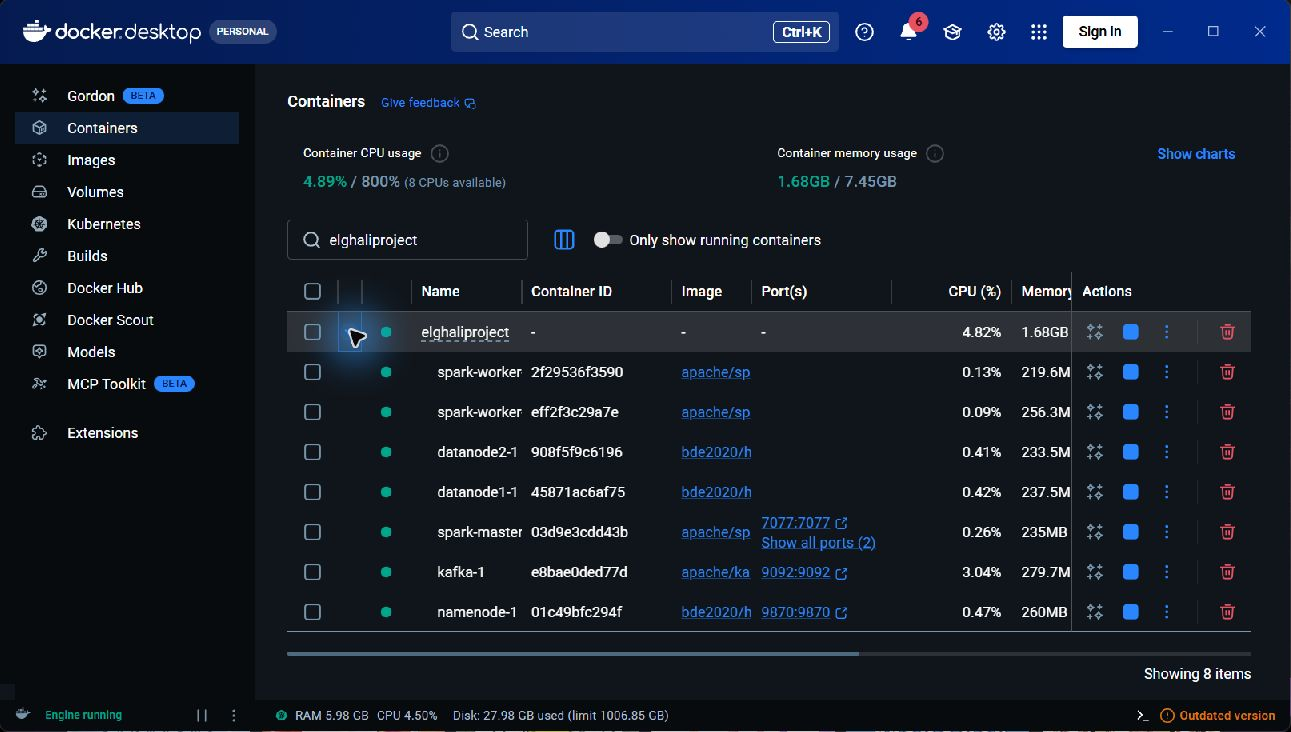
\includegraphics[width=\linewidth]{docs/figures/docker_services.png}
\caption{Docker Desktop après le démarrage : les sept services du projet sont actifs. Capture d'écran prise le 9 novembre 2026.}
\end{figure}

\begin{figure}[htbp]
\centering
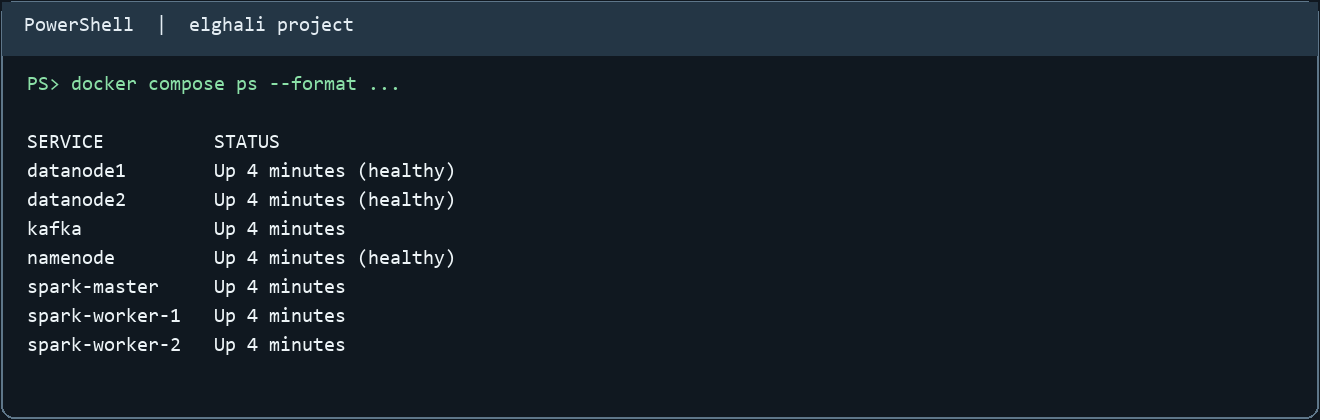
\includegraphics[width=0.92\linewidth]{docs/figures/terminal_docker_ps.png}
\caption{Sortie de \texttt{docker compose ps} enregistrée lors du même essai.}
\end{figure}

\section{Premier envoi dans Kafka}

Le producteur Python écrit d'abord un fichier JSONL. Avec l'option \texttt{--publish}, il envoie ensuite chaque ligne dans \texttt{youtube.videos.raw}, en utilisant \texttt{video\_id} comme clé. Une fixture de trois vidéos fictives permet de faire ce test sans consommer de quota Google. Les valeurs de cette fixture ne représentent aucune vidéo réelle.

\begin{figure}[htbp]
\centering
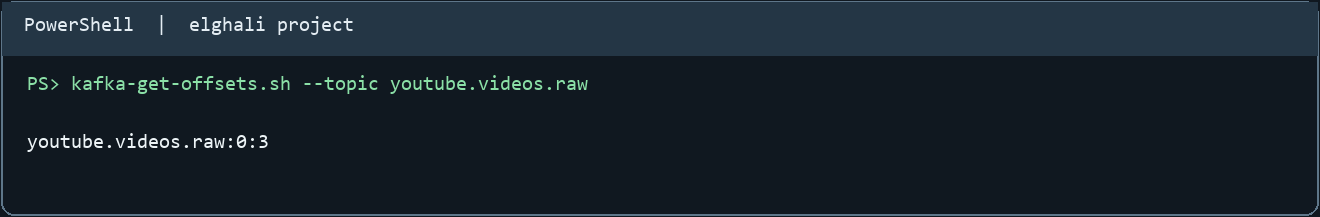
\includegraphics[width=0.83\linewidth]{docs/figures/terminal_kafka_offsets.png}
\caption{Offset final du topic Kafka après l'envoi de trois événements dans la partition 0. Sortie de commande conservée pour le rapport.}
\end{figure}

Le collecteur a bien écrit trois lignes JSONL et Kafka a reçu trois messages. La validation de Compose et les tests unitaires du collecteur ont réussi, notamment la pagination, la lecture du fichier \texttt{.env} et le cas d'une statistique manquante. Côté infrastructure, le NameNode a vu deux DataNodes actifs et l'interface du master Spark deux workers actifs.

Au démarrage, la commande du service Spark était mal transmise à \texttt{bash -lc} par Compose. Nous avons corrigé la forme de \texttt{command} puis relancé les services. Sur le poste de test, \texttt{kafka-python} 2.0.2 ne s'importait pas avec Python 3.14 ; le producteur utilise maintenant la version 3.0.13. Ces deux problèmes ont été détectés pendant l'essai, avant le traitement batch.

\section{Mode opératoire retenu}

Le démarrage se fait depuis la racine du dépôt avec \texttt{docker compose up -d}. La commande \texttt{docker compose ps} permet de repérer immédiatement un service arrêté ou en cours d'initialisation. Nous vérifions ensuite le rapport du NameNode avec \texttt{hdfs dfsadmin -report} et le nombre de workers sur l'interface du master Spark. Il faut attendre que les deux DataNodes soient inscrits avant d'écrire dans HDFS avec une réplication de 2.

Le topic est créé avec une seule partition et un facteur de réplication Kafka de 1, car le cluster de démonstration ne possède qu'un broker. Cette valeur ne concerne pas la réplication HDFS, qui reste à 2. Pour publier la fixture, la commande du README est \texttt{python -m ingestion.youtube\_batch --fixture data/demo\_videos.jsonl --publish}. Nous contrôlons ensuite l'offset final de la partition : il vaut 3 après trois messages et un topic initialement vide.

Après cet essai, une clé API a été placée dans \texttt{.env}. Une première collecte restreinte a permis de tester l'accès aux données réelles. Le lot local a ensuite été remplacé par 1\,000 vidéos issues des requêtes \og big data \fg{} et \og apache spark \fg{}, enregistrées dans \texttt{data/youtube\_real.jsonl}. La clé ne doit pas être ajoutée à Git. Les statistiques publiques peuvent changer ; chaque collecte doit donc être datée, et les données stockées actualisées ou supprimées selon les règles de l'API. Une recherche YouTube n'est pas un échantillonnage aléatoire : les résultats dépendent de la requête et du classement de l'API.

\section{Bilan de la semaine}

Le jalon technique de la première semaine est atteint : cluster démarré et événements publiés dans Kafka. Le jeu fictif a servi à l'essai initial, puis l'API a fourni un petit lot réel. Il reste à obtenir la validation du sujet et à répéter les relevés pour disposer d'un historique temporel. La répartition des tâches entre les trois membres sera consignée par le groupe avant la remise finale ; aucune attribution individuelle n'est déduite des seuls fichiers du dépôt.

\smallskip
{\small\textbf{Sources :} fiche de projet de Pr. El Ghali Btihal ;
\href{https://developers.google.com/youtube/data/reference/rest/v3/search/list}{YouTube \texttt{search.list}} ;
\href{https://developers.google.com/youtube/data/reference/rest/v3/videos/list}{YouTube \texttt{videos.list}} ;
\href{https://developers.google.com/youtube/terms/developer-policies}{règles de conservation des données API}.}

\end{document}
